\documentclass[a4paper,twoside,french,11pt]{book}
\usepackage[T1]{fontenc}
\usepackage{graphicx}
\usepackage[french]{babel}
\usepackage{times}
\usepackage{url}
\usepackage[utf8]{inputenc}
\usepackage{amsmath}
\usepackage{latexsym}
\usepackage{color}
\usepackage{listingsutf8}
\usepackage{xspace}
\usepackage[makeindex]{imakeidx}
\usepackage{hyperref}
\usepackage[toc,nonumberlist]{glossaries}
\usepackage[missing=Informations\ de\ version\ indisponibles]{gitinfo}
%\usepackage[nottoc]{tocbibind}
\sloppy

\makeindex[options= -s introgitindex.ist]
\makeglossaries

\addtolength{\topmargin}{-2cm}
\addtolength{\textheight}{+3cm}
\addtolength{\oddsidemargin}{-0,5cm}
\setlength{\evensidemargin}{\oddsidemargin}
\addtolength{\textwidth}{+3cm}

%\renewcommand\section{\@startsection {section}{1}{\z@}%
%	{-3.5ex \@plus -1ex \@minus -.2ex}%
%	{2.3ex \ at plus.2ex}%
%	{\reset@font\Large\bfseries}}

\lstset{
  language=bash,
  % backgroundcolor=\color[rgb]{0.91,0.91,0.95}, %bleu
  % backgroundcolor=\color[rgb]{0.89,0.93,0.89}, %vert
  backgroundcolor=\color{white},
  basicstyle=\scriptsize\ttfamily,
  % numbers=none,
  numberstyle=\footnotesize,
  numbersep=5pt,
  stringstyle=\ttfamily,
  showstringspaces=false,
  frame=tb,
  tabsize=2,
  % captionpos=t,
  morecomment=[l]{//},
  columns=flexible,
  inputencoding=utf8/latin1,
  % escapeinside={/*@}{@*/}
  extendedchars=\true,
  literate={ù}{{\`u}}1 {é}{{\'e}}1 {è}{{\`e}}1 {ê}{{\^e}}1 {â}{{\^a}}1 {û}{{\^u}}1 {Ç}{{\c C}}1 {à }{{\`a} }2
}

\makeatletter
\renewcommand\section{\@startsection
  {section}{1}{1cm}%name, level, indent
  {1.5\baselineskip}%             beforeskip
  {1\baselineskip}%            afterskip
  {\normalfont\Large\bfseries}}% style
  
\renewcommand\subsection{\@startsection
  {subsection}{2}{2cm}%name, level, indent
  {-\baselineskip}%             beforeskip
  {0.3\baselineskip}%            afterskip
  {\normalfont\normalsize\itshape\bfseries}}% style
  
\renewcommand\subsubsection{\@startsection
  {subsubsection}{3}{2.5cm}%name, level, indent
  {-\baselineskip}%             beforeskip
  {0.3\baselineskip}%            afterskip
  {\normalfont\normalsize\itshape\bfseries}}% style

\newlength{\drop}
\newcommand*{\titleIntroGit}{\begingroup
\drop = 0.2\textheight
\centering
\vspace*{\drop}
{\Huge \textsc{\@title}}\\[\baselineskip]
{\Huge \textsc{\subtitle}}\\[12\baselineskip]
{\Large \textsc{\maintainer}}\\[\baselineskip]
{\large \texttt{\url{\maintainerurl}}}\\%[\baselineskip]
{\large \href{mailto:\maintainermail}{\texttt{\maintainermail}}}\par
\vfill
{\Large Version \currentVersion}\par
\endgroup}

\g@addto@macro\@floatboxreset\centering
\makeatother

%Tableau de versionning
\newenvironment{versions}%
    {\vspace{0cm}\begin{table}[b]\begin{flushright}\begin{tabular}{l@{\hspace{0.5cm}}c@{\hspace{0.5cm}}r}\hline}%
    {\end{tabular}\end{flushright}\end{table}}

% Glossaire

\longnewglossaryentry{depot}
{
name=Dépôt,
sort=Depot,
}
{TODO}

\longnewglossaryentry{gestionVersions}
{
name=Gestion de versions,
sort=Gestion de versions
}
{Ensemble de fonctionnalités permettant un travail collaboratif sur un projet via la gestion des différents dépôts du projet, de son historique, de ses différentes versions et variantes, ainsi que des contributions concurrentes des différents participants et des conflits associés.}

\longnewglossaryentry{historique}
{
name=Historique,
sort=Historique
}
{Ensemble des révisions d'un projet, organisé sous forme d'un graphe de dépendance orienté et acyclique, permettant une représentation de la succession temporelle des modifications suivant un ordre partiel.}

\longnewglossaryentry{revision}
{
name=Révision,
sort=Revision
}
{Ensemble identifiable et atomique de modifications liées par une certaine unité sémantique, portant sur un ou plusieurs fichiers, réalisées par un même contributeur identifié, explicitement introduites dans un projet, accompagnées d'un message explicatif et d'autres méta-données, comme la date.}

\longnewglossaryentry{vcs}
{
  name=Système de gestion de versions,
  sort=Systeme de gestion de versions,
  plural=Systèmes de gestion de versions
}
{TODO}

% Redirections
\longnewglossaryentry{commit}
{
name={\it Commit\/},
sort=Commit
}
{{\it voir\/} Révision}
\longnewglossaryentry{repository}
{
  name={\it Repository\/},
  sort=Repository,
  plural=Repositories
}
{{\it voir\/} Dépôt}

\begin{document}
\pagestyle{empty}
\bibliographystyle{alpha}

\newcommand{\maintainer}{Guillaume Piolle}
\newcommand{\maintainerurl}{http://guillaume.piolle.fr/}
\newcommand{\maintainermail}{guillaume.piolle@centralesupelec.fr}
\newcommand{\currentVersion}{0.0}
  
\title{Gestion de versions}
\newcommand{\subtitle}{Introduction à Git}
\author{\maintainer}
\date{}

\titleIntroGit

{\small
  \par\vspace*{\fill}

  \paragraph*{Source}

  Ce document a été initialement publié sur la plate-forme GitHub, à
  l'adresse suivante~:\\
  \centerline{\url{https://github.com/Eusebius/IntroductionGit}}

  \paragraph*{Version}

  \currentVersion\
  (commit \gitAbbrevHash\ du \gitCommitterDate)
  
  \paragraph*{Licence}

  Ce document est publié sous la licence \textit{GNU General Public
    License v2.0}. Le texte complet peut en être trouvé ici~:\\
  \centerline{\url{https://www.gnu.org/licenses/old-licenses/gpl-2.0.fr.html}}

  C'est une licence libre, au sens de la \textit{Free Software
    Foundation}, qui autorise quiconque à réutiliser ce document pour
  quelque usage que ce soit, y compris les usages commerciaux et la
  création d'\oe uvres dérivées, à condition que celles-ci soient
  elles-mêmes publiées sous la même licence.

  \paragraph*{Comment contribuer à ce document~?}

  N'importe qui peut proposer une contribution directe à ce document
  sous la forme d'un \textit{pull request} sur le dépôt GitHub de la
  publication initiale. Le ou les gestionnaires du dépôt décident
  seuls de l'intégration des propositions dans le dépôt principal.

  Les commentaires, suggestions d'évolution, signalements de coquilles
  ou d'erreurs\ldots peuvent être directement soumis sur GitHub sous
  forme d'\textit{issues}.

  En vertu de la licence utilisée, n'importe qui peut également créer
  une version librement dérivée (\textit{fork}) de ce document, à
  condition de la publier sous la même licence.

  \paragraph*{Liste des contributeurs}
  Les personnes physiques suivantes ont contribué à la conception de
  ce document, librement et en l'absence d'instructions d'aucune
  sorte~; elles sont les seuls détenteurs des droits d'auteur
  associés à ce document~:
  \begin{itemize}
  \item Guillaume Piolle \texttt{<guillaume.piolle@centralesupelec.fr>}.
  \end{itemize}

  \begin{versions}
    v0.0 & GP & 22/11/13
  \end{versions}
}

\frontmatter

\chapter*{Avant-propos}
\thispagestyle{empty}

TODO \gls{vcs} qsdf

% TODO avant-propos, objectifs et philosophie du document, utilisation
% de termes anglais
% Commandes et noms de fichiers en tt
% Guide d'autoformation ?

\mainmatter
\pagestyle{headings}
\setcounter{page}{1}
\tableofcontents

% Aide-mémoire pour l'indexation
% Texte\index{Entree non accentuee@Entrée accentuée!sous-entrée!sous-sous-entrée}
% \index{Entrée|see{Entrée pointée par la redirection}}

% Redirections d'index
\index{arch|see{GNU arch}}
\index{commit@\textit{commit}|see{révision}}
\index{copy-modify-merge@\textit{copy-modify-merge}|see{fusion}}
\index{gestionnaire de versions|see{système de gestion de versions}}
\index{gitignore@\texttt{gitignore}|see{\texttt{.gitignore}}}
\index{Helix|see{Perforce Helix}}
\index{IDE|see{environnement de développement intégré}}
\index{lock-modify-unlock@\textit{lock-modify-unlock}|see{verrouillage}}
\index{repository@\textit{repository}|see{dépôt}}
\index{revision control@\textit{revision control}|see{gestion de versions}}
\index{SourceSafe|see{Microsoft Visual SourceSafe}}
\index{SVN|see{Subversion}}
\index{VCS|see{système de gestion de versions}}
\index{version control@\textit{version control}|see{gestion de versions}}
\index{VSS|see{Microsoft Visual SourceSafe}}

\chapter{Introduction non facultative}\label{chapIntro}

Ce chapitre présente les besoins et les concepts de la gestion de
versions d'une manière générale, ainsi qu'un aperçu des différentes
familles de systèmes de gestion de versions. Il se focalise ensuite sur
Git, qui sera l'objet du reste de cet ouvrage, pour en expliquer la
philosophie et le modèle de fonctionnement.

\section{Les besoins du génie logiciel}

La \textbf{gestion de versions}\index{Gestion de versions} (en anglais
\textit{version control} ou \textit{revision control}) est une
fonctionnalité, ou plutôt une famille de fonctionnalités, qui trouve
son origine dans les besoins du développement logiciel en
équipe. Plusieurs développeurs travaillant ensemble sur le même
ensemble de fichiers, même si les domaines d'intervention de chacun
sont clairement définis, doivent nécessairement trouver un moyen de
collaborer de manière constructive, sans que les contributions des uns
ne deviennent un souci pour les autres. La gestion de version, en
s'appuyant sur un \textbf{historique}\index{historique} raisonné du
développement, a pour vocation de répondre à l'ensemble des besoins
détaillés ci-après.

\subsection{Gestion des instances du projet}

Les outils de gestion de versions doivent permettre d'identifier
plusieurs instances (éventuellement à des stades de développement
différents) du même projet. Ces instances peuvent correspondre,
suivant les cas, à l'espace de travail direct d'un développeur ou d'un
ensemble de développeurs, à une instance de référence commune partagée
par tous ou par un sous-groupe des développeurs, à une instance de
mise à disposition du public des versions stables du projet\ldots

Ces instances sont désignées sous le terme générique de
\textbf{dépôt}\index{depot@dépôt} (\textit{repository} en
anglais). Chaque dépôt est une représentation du projet. Suivant les
choix d'organisation et le système de gestion de versions utilisé, un
dépôt peut représenter le projet dans son intégralité ou bien
seulement un sous-ensemble, l'intégralité de son historique ou bien
seulement une partie. Un dépôt peut être
\textbf{local}\index{depot@dépôt!local}, c'est-à-dire situé sur la
machine de développement d'un des contributeurs (sans être
nécessairement confondu avec l'espace de travail direct du
développeur), ou bien \textbf{distant}\index{depot@dépôt!distant},
déporté sur un serveur accessible via le réseau.

\subsection{Gestion de l'historique}

La gestion de versions est un moyen de conserver une trace de
l'historique du projet, sous la forme d'un ensemble de
\textbf{révisions}\index{revision@révision} (\textit{commits} en
anglais). Une révision est un ensemble atomique et identifiable de
modifications liées par une certaine unité sémantique, portant sur un
ou plusieurs fichiers, réalisées par un même contributeur identifié,
explicitement introduites dans le projet, accompagnées d'un message
explicatif et d'autres méta-données, comme la date\footnote{Dans
  certains systèmes, comme par exemple Overleaf\index{Overleaf}, qui
  est une surcouche web de Git pour la rédaction collaborative
  (\url{https://www.overleaf.com/}), les révisions peuvent être
  générées automatiquement, de manière périodique ou à chaque
  modification élémentaire. Dans ce cas, une révision peut n'avoir ni
  unité sémantique ni message explicatif, ce qui limite forcément
  l'utilité de l'historique résultant. D'autre part, l'unicité
  sémantique des révisions est une propriété qui, si elle est
  désirable, dépend en grande partie de la bonne volonté des
  contributeurs\ldots}. L'atomicité signifie que les modifications
d'une même révision sont toutes appliquées ensemble au projet (ou
qu'aucune ne l'est), sans qu'une modification provenant d'une autre
révision puisse venir interférer ni que le projet puisse se retrouver
dans un état incohérent (avec une révision partiellement
appliquée)\footnote{Il existe des systèmes de gestion de versions dans
  lesquels les révisions ne sont pas atomiques. Nous ne les
  mentionneront pas ici, dans l'espoir que leur nom disparaisse à
  jamais de la mémoire collective et de l'histoire de l'informatique
  (pour plus de détails sur les bonnes pratiques du révisionnisme avec
  Git, les nostalgiques du Ministère de la Vérité \cite{Orwell}
  pourront étudier avec intérêt la section~\ref{secRevisionnisme}).}.
Par abus de langage, le terme de révision ou de \textit{commit}
désigne également l'état du projet après application des modifications
en question.

Dans le cas le plus simple, un historique est une succession linéaire
de révisions, chacune s'appuyant sur la précédente
(figure~\ref{fig:historiqueLineaire}). Dans la majorité des cas,
cependant, il en ira tout autrement\ldots\ Dans la syntaxe graphique
que nous adoptons pour les historiques, les cercles représentent les
révisions et les flèches représentent les dépendances entre
ces révisions. Le sens de ces flèches n'est donc pas le sens d'écoulement
du temps (qui va de la gauche vers la droite pour un historique
linéaire)~: le fait que la révision $E$ pointe vers la révision $D$
($D \leftarrow E$) veut dire que $E$ s'appuie sur $D$, et donc qu'elle
vient après cette dernière dans le processus de conception.

\begin{figure}[h!]
  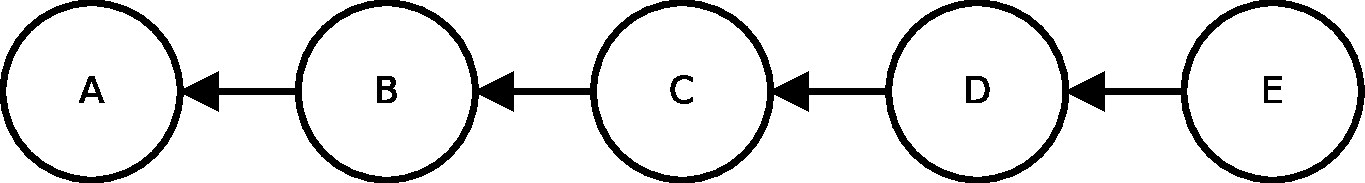
\includegraphics[width=10cm]{figures/historiqueLineaire}
  \caption{Exemple d'historique de développement linéaire, constitué
    de cinq révisions successives.\label{fig:historiqueLineaire}}
\end{figure}


L'historique a lui-même différentes utilités, au-delà de ce rôle de
représentation temporelle, notamment parce qu'il est généralement
navigable, voire cherchable. Suivant les systèmes, l'historique peut
permettre de déterminer~:
\begin{itemize}
\item La date d'introduction d'une révision donnée~;
\item L'auteur d'une révision donnée~;
\item Les modifications apportées par une révision donnée~;
\item Les causes et motivations d'une modification (si la révision
  concernée a été correctement documentée)~;
\item La révision ayant introduit une fonctionnalité, un
  bogue\index{bogue}, une régression\index{regression@régression}, une
  vulnérabilité\ldots
\item \ldots
\end{itemize}

\subsection{Intégration de contributions dans un même projet} % TODO 

Les différentes personnes participant à un même projet doivent pouvoir
voir leurs contributions individuelles intégrées au projet, idéalement
de manière fluide, transparente et indolore.

Intégration des contributions de différentes personnes dans un
  même projet, en permettant la résolution des incohérences pouvant
  survenir entre des modifications concurrentes~;

% Développement de fonctionnalités en parallèle, fusion, résolution de conflits
% Notion de conflit
\index{conflit}


\subsection{Gestion de variantes différentes du même projet} % TODO 

Possibilité de créer et de maintenir simultanément des variantes du
projet, par exemple pour expérimenter l'utilisation de nouvelles
technologies, le développement de nouvelles fonctionnalités ou la mise
en place d'une nouvelle organisation~;

\section{Systèmes de gestion de version} %TODO
\index{systeme de gestion de versions@système de gestion de versions}

% fichiers texte et fichiers binaires

\subsection{Systèmes centralisés} %TODO
\index{systeme de gestion de versions@système de gestion de versions!centralises@centralisé}
% TODO CVS
\index{CVS}
% TODO Subversion
\index{Subversion}
% TODO Visual SourceSafe
\index{Visual SourceSafe}
% TODO Perforce Helix
\index{Perforce Helix}
% TODO VSTS (Visual Studio Team Services)
\index{Visual Studio Team Services}

\subsection{Systèmes décentralisés} %TODO
\index{systeme de gestion de versions@système de gestion de versions!decentralises@décentralisé}
% TODO Git
\index{Git}
% TODO GNU arch
\index{GNU arch}
% TODO Mercurial
\index{Mercurial}
% TODO BitKeeper
\index{BitKeeper}
% TODO Bazaar
\index{Bazaar}
% TODO Darcs
\index{Darcs}
% TODO Veracity
\index{Veracity}
% TODO VSTS (Visual Studio Team Services)
\index{Visual Studio Team Services}

\section{Le modèle de Git} %TODO
% TODO philosophie, différents éléments du modèle

\subsection{Principes et philosophie} %TODO

\subsection{Git sur les différents systèmes d'exploitation}\label{GitOS} %TODO
\index{Windows}
\index{Linux}
\index{macOS}

\subsection{Les différents éléments du modèle} %TODO

\index{.git@\texttt{.git}}

\index{SHA1}
% TODO Expliquer en footnote que Git utilise SHA1 comme un code de
% détection d'erreur et non comme un algorithme de hachage
% cryptographique. En théorie, il est possible de falsifier le contenu
% d'un commit Git utilisant SHA1, par exemple pour y insérer du code
% malveillant, en conservant le même haché. Subversion utilise SHA1
% également, et les PDF en collision le faisaient planter, nécessitant
% un correctif. Sauf que Git utilise également SHA1 pour signer les
% commits, et là évidemment ça pose un problème d'authenticité et plus
% seulement d'intégrité.
% http://www.zdnet.fr/actualites/collision-sha-1-linus-torvalds-se-veut-rassurant-sur-git-39849070.htm
% https://twitter.com/matthew_d_green/status/835864260240683009/photo/1

\subsection{Structure d'un dépôt} %TODO
\index{depot@dépôt}
\index{depot@dépôt!local}
% TODO notion de référence

\subsection{Modèle de configuration} %TODO
\index{configuration}
\index{git@\texttt{git}!config@\texttt{config}}
\index{global@\texttt{global}}
\index{system@\texttt{system}}
\index{local@\texttt{local}}
% TODO global / system / local, principales variables

\chapter{Le minimum à maîtriser pour survivre avec Git}\label{chapMinimum} % TODO
% TODO obtenir de l'aide
\index{git@\texttt{git}!help@\texttt{help}}

\section{Enregistrer et lister des modifications} %TODO
% TODO staging, add, rm commit, log
\index{git@\texttt{git}!init@\texttt{init}}
\index{git@\texttt{git}!commit@\texttt{commit}}
\index{git@\texttt{git}!log@\texttt{log}}
\index{historique}
\index{git@\texttt{git}!add@\texttt{add}}
\index{git@\texttt{git}!rm@\texttt{rm}}

\section{Gestion des fichiers non versionnés} % TODO
% TODO .gitignore
\index{ignorer un fichier}
\index{.gitignore@\texttt{.gitignore}}

\section{Gestion des branches} % TODO
% TODO .gitignore
\index{branche}
\index{git@\texttt{git}!branch@\texttt{branch}}
\index{git@\texttt{git}!checkout@\texttt{checkout}}

\section{Travailler avec un dépôt distant} % TODO 
% TODO clone, push, pull, fetch, merge
\index{depot@dépôt!distant}
\index{git@\texttt{git}!clone@\texttt{clone}}
\index{git@\texttt{git}!push@\texttt{push}}
\index{git@\texttt{git}!pull@\texttt{pull}}
\index{git@\texttt{git}!fetch@\texttt{fetch}}
\index{git@\texttt{git}!merge@\texttt{merge}}

\section{Résolution des conflits} %TODO

\index{git@\texttt{git}!merge@\texttt{merge}}
\index{conflit}
% La figure~\ref{fig:conflitGit} illustre l'apparition d'un conflit au
% cours d'un développement en équipe. À un instant donné, le dépôt
% commun aux deux développeurs contient les révisions $A$ et $B$. Le
% premier développeur va commencer un travail sur cette base, et
% produire les révisions $C1$ et $D1$.

% \begin{figure}[h!]
%   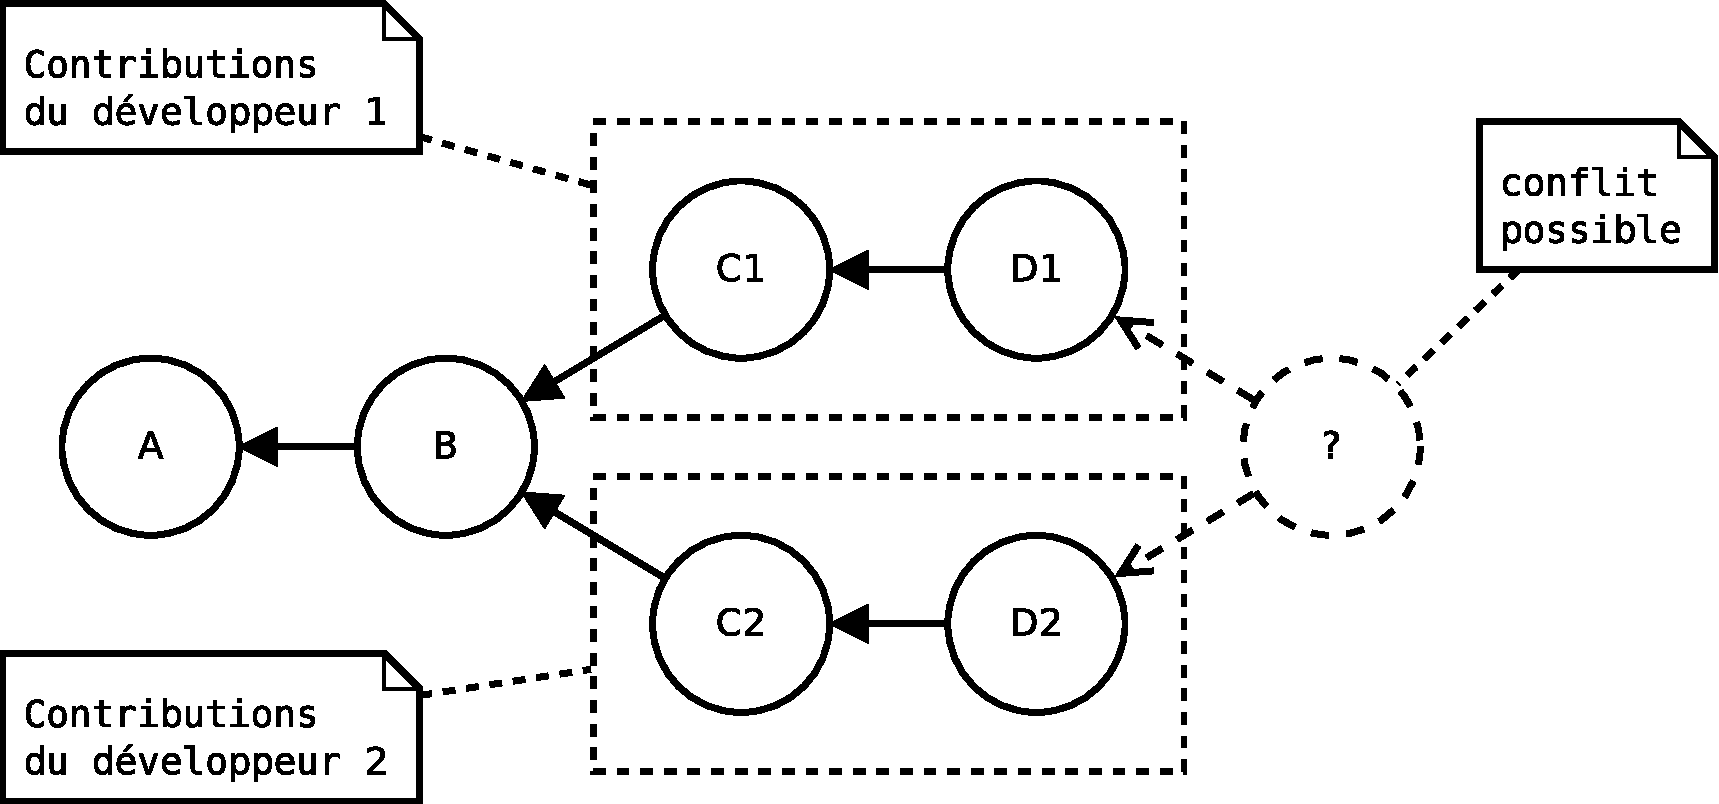
\includegraphics[width=12cm]{figures/conflitGit}
%   \caption{Apparition d'un conflit potentiel entre les contributions
%     de deux développeurs.\label{fig:conflitGit}}
% \end{figure}

\section{Gestion des \textit{tags}} % TODO 
% TODO navigation dans l'historique, reset, revert
% TODO branches, navigation entre branches
% TODO fusion et gestion des conflits
\index{tag@\textit{tag}}
\index{git@\texttt{git}!tag@\texttt{tag}}
\index{git@\texttt{git}!reset@\texttt{reset}}
\index{git@\texttt{git}!revert@\texttt{revert}}
\index{historique}
\index{git@\texttt{git}!branch@\texttt{branch}}
\index{branche}
\index{git@\texttt{git}!checkout@\texttt{checkout}}

\chapter{Aspects plus avancés}\label{chapAvance} % TODO

% TODO hooks et pratiques relatives aux hooks ?
% TODO verrouillage dans Git ? Seulement dans Git LFS ?

\section{Politiques de développement et de collaboration} %TODO
% TODO gestion des branches et des dépôts
\index{branche}
\index{depot@dépôt!distant}
\index{depot@dépôt!upstream@\textit{upstream}}
\index{depot@dépôt!downstream@\textit{downstream}}

\section{Le \textit{stash}} %TODO
\index{git@\texttt{git}!stash@\texttt{stash}}

\section{\texttt{merge}, \texttt{squash} et \texttt{rebase}} %TODO trouver un meilleur titre

% TODO cf GitHub :
% https://help.github.com/articles/about-pull-request-merges/
% https://github.com/blog/2141-squash-your-commits
% https://github.com/edx/edx-platform/wiki/How-to-Rebase-a-Pull-Request
% TODO ajouter index

\section{Stratégies de fusion} % TODO
\index{git@\texttt{git}!merge@\texttt{merge}}
\index{strategie de fusion@stratégie de fusion}
\index{strategie de fusion@stratégie de fusion!ours@\texttt{ours}}
\index{strategie de fusion@stratégie de fusion!theirs@\texttt{theirs}}
\index{strategie de fusion@stratégie de fusion!octopus@\texttt{octopus}}

\section{Remaniement de l'historique}\label{secRevisionnisme}
\index{historique}
\index{git@\texttt{git}!cherry-pick@\texttt{cherry-pick}}
\index{git@\texttt{git}!filter-branch@\texttt{filter-branch}}
\index{git@\texttt{git}!commit@\texttt{commit}!amend@\texttt{-{}-amend}}
% TODO cherry-pick, réécriture d'historique, amend

\section{Sous-modules} % TODO
\index{sous-module}
% TODO présenter brièvement les autres méthodes pour intégrer plusieurs projets

\chapter{Pratiques usuelles}\label{chapPratiques} % TODO

\section{Granularité des révisions} %TODO
\index{revision@révision}

\section{Versionnement sémantique} 
% TODO \cite{SemVer}
\index{versionnement!semantique@sémantique}

\section{Organisation de dépôts multiples} % TODO duplicat avec Politiques de développement et de collaboration ?
% TODO notion de upstream et compagnie, différentes stratégies
% TODO collaboration par pull request
\index{depot@dépôt!distant}
\index{depot@dépôt!upstream@\textit{upstream}}
\index{depot@dépôt!downstream@\textit{downstream}}
\index{pull request@\textit{pull request}}

\section{Organisations des branches}\label{secOrgBranches} %TODO
% TODO branches par version, par fonctionnalités, par sous-projets,
% gestion des tags...

% main branch, maintenance branch (bugfixes), development/feature branches (disruptive changes), release branch (frozen code)
% branche master protégée (par des tests, par un contributeur autorisé...), ou bien développements au quotidiens dans la branche master
\index{branche}
\index{tag@\textit{tag}}

\section{Interaction avec les contributeurs externes} %TODO
% TODO forking, patches, pull requests

\chapter{Lien avec d'autres logiciels et plates-formes}\label{chapLiens} % TODO
% TODO bien préciser que les listes ne sont pas exhaustives

\section{Forges en ligne} % TODO
% TODO sourceforge, github, gitlab, bitbucket, gforge...
\index{forge}
\index{SourceForge}
\index{GitHub}
\index{GitLab}
\index{BitBucket}
\index{GForge}

\section{Environnements de développement} % TODO
% TODO Eclipse, Netbeans
\index{environnement de developpement integre@environnement de développement intégré}
\index{Eclipse}
\index{Netbeans}

\section{Intégration continue et assurance qualité}\label{secCI} % TODO
% TODO Code Climate, Jenkins, Travis...
\index{intégration continue}
\index{assurance qualité}
\index{couverture}
\index{test}
\index{CodeClimate}
\index{Jenkins}
\index{Travis CI}

\chapter{Les petites recettes pratiques qui sauvent la vie} % TODO

\section{Alias pour l'affichage de l'historique} %TODO
\index{alias}
\index{historique}
\index{git@\texttt{git}!log@\texttt{log}}

\section{Renoncer aux changements en cours} %TODO
\index{git@\texttt{git}!reset@\texttt{reset}}
\index{git@\texttt{git}!stash@\texttt{stash}}
% TODO les subtilités de reset

\section{Trouver l'origine d'un bogue} % TODO
\index{git@\texttt{git}!blame@\texttt{blame}}
\index{git@\texttt{git}!bisect@\texttt{bisect}}
\index{debogage@débogage}
\index{bogue}
\index{historique}
% TODO git blame, git bisect. Remonter dans la section sur l'historique ?

\section{Maintenir une différence constante entre deux branches} % TODO
\index{strategie de fusion|stratégie de fusion!ours@\texttt{ours}}

\appendix

\glsaddall
\nocite{*}

\cleardoublepage
\phantomsection
\addcontentsline{toc}{chapter}{\glossaryname}
\printglossaries

\cleardoublepage
\phantomsection
\addcontentsline{toc}{chapter}{\indexname}
\printindex

\cleardoublepage
\phantomsection
\addcontentsline{toc}{chapter}{\bibname}
\bibliography{introgit}

\end{document}


%%% Local Variables:
%%% mode: latex
%%% TeX-master: t
%%% ispell-local-dictionary: "francais"
%%% End: 